    In Einstein’s theory, time is defined operationally through the arrival and departure of light signals. Simultaneity is not absolute, but constructed by coordinating photon trajectories between clocks. This makes time a relational concept—dependent on the motion of observers and the invariance of light speed.

    \begin{table}[h!]
        \centering
        \begin{tabular}{|c|c|c|c|}
            \hline
            \textbf{Theory} & \textbf{Time} & \textbf{Simultaneity} & \textbf{Defined By} \\
            \hline
            Newton & Absolute & Universal & External flow of time \\
            Einstein (SR/GR) & Relative & Frame-dependent & Light signal coordination \\
            VAM & Layered (N, $\tau$, $S(t)$) & Phase-coherent & Vortex swirl phase $\Omega(r)$ \\
            \hline
        \end{tabular}
        \caption{Comparison of time and simultaneity in Newtonian, Einsteinian, and VAM frameworks.}
    \end{table}

    In contrast, the Vortex Æther Model grounds time in the internal dynamics of the medium itself. Absolute æther time \( N \) flows uniformly, while local time \( \tau \) and swirl clock time \( S(t) \) emerge from the rotational energy and helicity of vortex structures. Simultaneity is no longer a matter of synchronization via photons—it is encoded in the shared phase coherence of knotted circulation. In this sense, VAM replaces relativistic light-clock simultaneity with a topologically grounded, energetically conserved temporal ontology.



\begin{figure}[htbp]
      \centering
    \scriptsize
        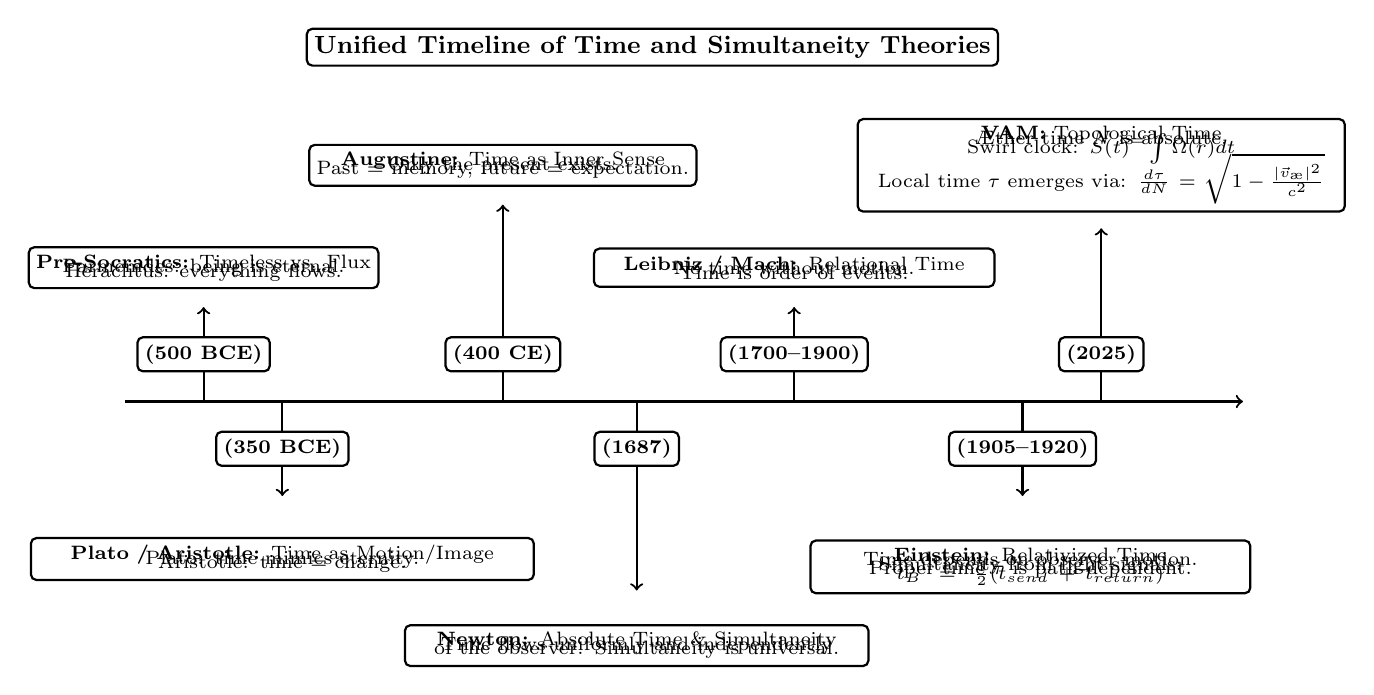
\begin{tikzpicture}
        \scriptsize
        % Timeline base
        \draw[->, thick] (-1,0) -- (13.2,0);

        % Arrows above timeline (short, as requested)
        \draw[->, thick] (0,0) -- (0,1.2);       % Pre-Socratics
        \draw[->, thick] (3.8,0) -- (3.8,2.5);   % Augustine
        \draw[->, thick] (7.5,0) -- (7.5,1.2);   % Einstein
        \draw[->, thick] (11.4,0) -- (11.4,2.2); % VAM

        % Arrows below timeline (short, as requested)
        \draw[->, thick] (1.0,0) -- (1.0,-1.2);     % Plato/Aristotle
        \draw[->, thick] (5.5,0) -- (5.5,-2.4);     % Newton
        \draw[->, thick] (10.4,0) -- (10.4,-1.2);     % Leibniz/Mach

            %--- Root title cards (above timeline) ---
        \node[draw, thick, rounded corners=2pt, fill=white, align=center, font=\bfseries ] at (0, .6)   {(500 BCE)};
        \node[draw, thick, rounded corners=2pt, fill=white, align=center, font=\bfseries ] at (3.8, .6) {(400 CE)};
        \node[draw, thick, rounded corners=2pt, fill=white, align=center, font=\bfseries ] at (7.5, .6) {(1700--1900)};
        \node[draw, thick, rounded corners=2pt, fill=white, align=center, font=\bfseries ] at (11.4, .6){(2025)};

        %--- Root title cards (below timeline) ---
        \node[draw, thick, rounded corners=2pt, fill=white, align=center, font=\bfseries ] at (1.0,- .6) {(350 BCE)};
        \node[draw, thick, rounded corners=2pt, fill=white, align=center, font=\bfseries ] at (5.5,- .6) {(1687)};
        \node[draw, thick, rounded corners=2pt, fill=white, align=center, font=\bfseries ] at (10.4,- .6) {(1905--1920)};

            % Timeline label
        \node[draw, thick, fill=white, rounded corners=2pt, font=\small] at (5.7,4.5) {\textbf{Unified Timeline of Time and Simultaneity Theories}};

        % --- Pre-Socratics ---
        \node[draw, rounded corners=2pt, thick, align=center, fill=white] at (0,1.7) {
        \textbf{Pre-Socratics:} Timeless vs. Flux \\[-0.8em]
        Parmenides: being is eternal. \\[-0.8em]
        Heraclitus: everything flows.
        };

        % --- Augustine ---
        \node[draw, rounded corners=2pt, thick, align=center, fill=white] at (3.8,3.0) {
        \textbf{Augustine:} Time as Inner Sense \\[-0.8em]
        Only the present exists. \\[-0.8em]
        Past = memory, future = expectation.
        };

        % --- Leibniz / Mach ---
        \node[draw, rounded corners=2pt, thick, align=center, fill=white, text width=4.9cm] at (7.5,1.7) {
        \textbf{Leibniz / Mach:} Relational Time \\[-0.8em]
        No time without motion. \\[-0.8em]
        Time is order of events.
        };
        % --- VAM (modern) ---
        \node[draw, rounded corners=2pt, thick, align=center, fill=white, text width=6.0cm] at (11.4,3.0) {
        \textbf{VAM:} Topological Time \\[-0.8em]
        Æther time $N$ is absolute. \\[-0.6em]
        Swirl clock: $S(t)^\circlearrowleft = \int \Omega(r) dt$ \\[-0.6em]
        Local time $\tau$ emerges via: $ \frac{d\tau}{dN} = \sqrt{1 - \frac{|\vec{v}_\text{\ae}|^2}{c^2}}$

        };


        % --- Plato / Aristotle ---
        \node[draw, rounded corners=2pt, thick, align=center, fill=white, text width=6.2cm] at (1.0,-2) {
        \textbf{Plato / Aristotle:} Time as Motion/Image \\[-0.8em]
        Plato: time mimics eternity. \\[-0.8em]
        Aristotle: time = change.
        };



        % --- Einstein ---
        \node[draw, rounded corners=2pt, thick, align=center, fill=white, text width=5.4cm] at (10.5,-2.1) {
        \textbf{Einstein:} Relativized Time \\[-0.8em]
        Time depends on observer motion. \\[-0.8em]
        Simultaneity from light signals: \\[-0.8em]
        Proper time $\tau$ is path-dependent.\\[-0.8em]
        $t_B = \frac{1}{2}(t_{\text{send}} + t_{\text{return}})$
        };

        % --- Newton ---
        \node[draw, rounded corners=2pt, thick, align=center, fill=white, text width=5.7cm] at (5.5,-3.1) {
        \textbf{Newton:} Absolute Time \& Simultaneity \\[-0.8em]
        Time flows uniformly and independently \\[-0.8em]
        of the observer. Simultaneity is universal.
        };
         \end{tikzpicture}
        \caption{Fused history of time and simultaneity: from early philosophical views and Newton’s absolutes to Einstein’s relativistic structure and VAM’s layered, swirl-based temporality.}\label{fig:history-time-simultaneity}
\end{figure}

\resizebox{\textwidth}{!}{%
      \centering
    \scriptsize
    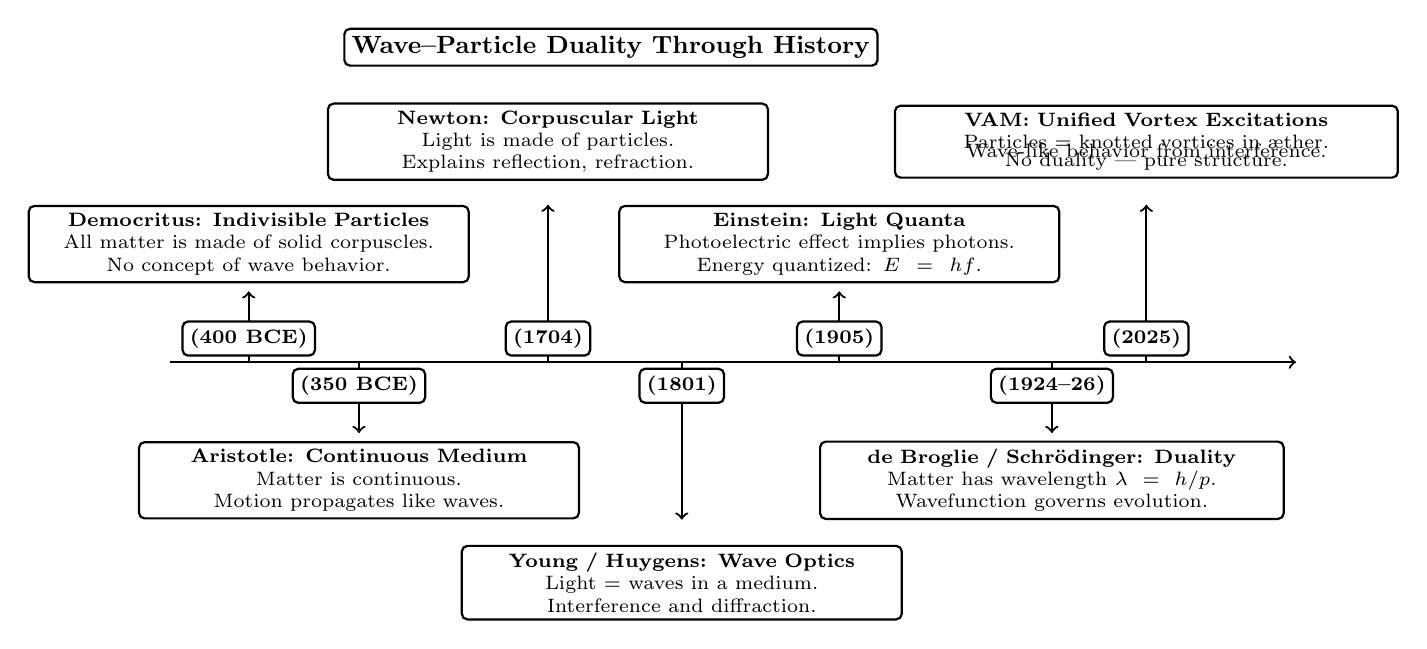
\begin{tikzpicture}
    \scriptsize

    % Timeline base
    \draw[->, thick] (-1,0) -- (13.3,0);

    % Arrows above timeline
    \draw[->, thick] (0,0) -- (0,0.9);       % Democritus
    \draw[->, thick] (3.8,0) -- (3.8,2.0);   % Newton
    \draw[->, thick] (7.5,0) -- (7.5,0.9);   % Einstein
    \draw[->, thick] (11.4,0) -- (11.4,2.0); % VAM

    % Arrows below timeline
    \draw[->, thick] (1.4,0) -- (1.4,-0.9);     % Aristotle
    \draw[->, thick] (5.5,0) -- (5.5,-2.0);     % Young/Huygens
    \draw[->, thick] (10.2,0) -- (10.2,-0.9);   % de Broglie

    % --- Date labels ---
    \node[draw, thick, rounded corners=2pt, fill=white, align=center, font=\bfseries ] at (0, .3)   {(400 BCE)};
    \node[draw, thick, rounded corners=2pt, fill=white, align=center, font=\bfseries ] at (3.8, .3) {(1704)};
    \node[draw, thick, rounded corners=2pt, fill=white, align=center, font=\bfseries ] at (7.5, .3) {(1905)};
    \node[draw, thick, rounded corners=2pt, fill=white, align=center, font=\bfseries ] at (11.4, .3){(2025)};

    \node[draw, thick, rounded corners=2pt, fill=white, align=center, font=\bfseries ] at (1.4,- .3) {(350 BCE)};
    \node[draw, thick, rounded corners=2pt, fill=white, align=center, font=\bfseries ] at (5.5,- .3) {(1801)};
    \node[draw, thick, rounded corners=2pt, fill=white, align=center, font=\bfseries ] at (10.2,- .3) {(1924--26)};

    % Timeline label
    \node[draw, thick, fill=white, rounded corners=2pt, font=\small] at (4.6,4.0) {\textbf{Wave–Particle Duality Through History}};

    % --- Democritus ---
    \node[draw, rounded corners=2pt, thick, align=center, fill=white, text width=5.4cm] at (0,1.5) {
    \textbf{Democritus: Indivisible Particles} \\% [-0.8em]
    All matter is made of solid corpuscles. \\% [-0.8em]
    No concept of wave behavior.
    };

    % --- Newton ---
    \node[draw, rounded corners=2pt, thick, align=center, fill=white, text width=5.4cm] at (3.8,2.8) {
    \textbf{Newton: Corpuscular Light} \\% [-0.8em]
    Light is made of particles. \\% [-0.8em]
    Explains reflection, refraction.
    };

    % --- Einstein ---
    \node[draw, rounded corners=2pt, thick, align=center, fill=white, text width=5.4cm] at (7.5,1.5) {
    \textbf{Einstein: Light Quanta} \\% [-0.8em]
    Photoelectric effect implies photons. \\% [-0.8em]
    Energy quantized: \( E = hf \).
    };

    % --- VAM ---
    \node[draw, rounded corners=2pt, thick, align=center, fill=white, text width=6.2cm] at (11.4,2.8) {
    \textbf{VAM: Unified Vortex Excitations} \\% [-0.8em]
    Particles = knotted vortices in æther. \\[-0.6em]
    Wave-like behavior from interference. \\[-0.6em]
    No duality — pure structure.
    };

    % --- Aristotle ---
    \node[draw, rounded corners=2pt, thick, align=center, fill=white, text width=5.4cm] at (1.4,-1.5) {
    \textbf{Aristotle: Continuous Medium} \\% [-0.8em]
    Matter is continuous. \\% [-0.8em]
    Motion propagates like waves.
    };

    % --- Young / Huygens ---
    \node[draw, rounded corners=2pt, thick, align=center, fill=white, text width=5.4cm] at (5.5,-2.8) {
    \textbf{Young / Huygens: Wave Optics} \\% [-0.8em]
    Light = waves in a medium. \\% [-0.8em]
    Interference and diffraction.
    };

    % --- de Broglie / Schrödinger ---
    \node[draw, rounded corners=2pt, thick, align=center, fill=white, text width=5.7cm] at (10.2,-1.5) {
    \textbf{de Broglie / Schrödinger: Duality} \\% [-0.8em]
    Matter has wavelength \( \lambda = h/p \). \\% [-0.8em]
    Wavefunction governs evolution.
    };

    \end{tikzpicture}
    \caption{\textbf{Intellectual trajectory of wave–particle duality:} from classical corpuscles and wave models to quantum dualities and beyond. VAM reframes the dichotomy by modeling all excitations as topologically structured vortices in a fluid æther. In this view, “particles” and “waves” are unified as geometric flow phenomena—dispensing with dualism in favor of pure structure.}\label{fig:WaveParticleDuality}
}
\begin{center}
\footnotesize
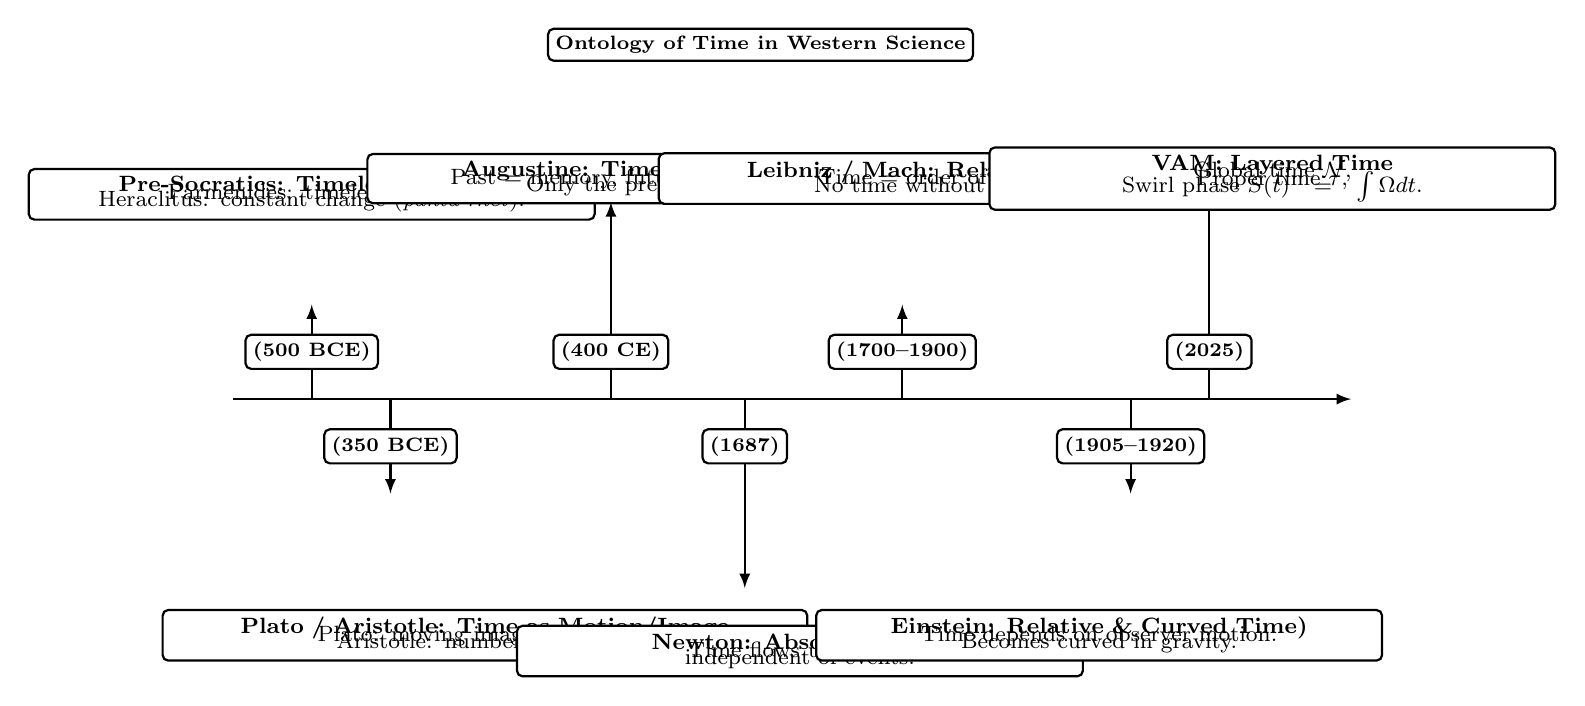
\begin{tikzpicture}[node distance=3.5cm, every node/.style={font=\footnotesize}, >=latex]
\scriptsize


% Timeline base
\draw[->, thick] (-1,0) -- (13.2,0);

% Arrows above timeline (short, as requested)
\draw[->, thick] (0,0) -- (0,1.2);       % Pre-Socratics
\draw[->, thick] (3.8,0) -- (3.8,2.5);   % Augustine
\draw[->, thick] (7.5,0) -- (7.5,1.2);   % Einstein
\draw[->, thick] (11.4,0) -- (11.4,3.0); % VAM

% Arrows below timeline (short, as requested)
\draw[->, thick] (1.0,0) -- (1.0,-1.2);     % Plato/Aristotle
\draw[->, thick] (5.5,0) -- (5.5,-2.4);     % Newton
\draw[->, thick] (10.4,0) -- (10.4,-1.2);     % Leibniz/Mach

    %--- Root title cards (above timeline) ---
\node[draw, thick, rounded corners=2pt, fill=white, align=center, font=\bfseries ] at (0, .6)   {(500 BCE)};
\node[draw, thick, rounded corners=2pt, fill=white, align=center, font=\bfseries ] at (3.8, .6) {(400 CE)};
\node[draw, thick, rounded corners=2pt, fill=white, align=center, font=\bfseries ] at (7.5, .6) {(1700--1900)};
\node[draw, thick, rounded corners=2pt, fill=white, align=center, font=\bfseries ] at (11.4, .6){(2025)};

%--- Root title cards (below timeline) ---
\node[draw, thick, rounded corners=2pt, fill=white, align=center, font=\bfseries ] at (1.0,- .6) {(350 BCE)};
\node[draw, thick, rounded corners=2pt, fill=white, align=center, font=\bfseries ] at (5.5,- .6) {(1687)};
\node[draw, thick, rounded corners=2pt, fill=white, align=center, font=\bfseries ] at (10.4,- .6) {(1905--1920)};

% Label (centered box)
\node[draw, thick, fill=white, rounded corners=2pt, font=\scriptsize] at (5.7,4.5) {\textbf{Ontology of Time in Western Science}};

% Ancient Greek: Parmenides / Heraclitus
\node[draw, rounded corners=2pt, thick, align=center, fill=white, text width=7cm] at (0,2.6) {
\textbf{Pre-Socratics: Timeless vs. Flux}  \\[-0.8em]
Parmenides: timeless being.  \\[-0.8em]
Heraclitus: constant change (\textit{panta rhei}).
};

% Plato / Aristotle
\node[draw, rounded corners=2pt, thick, align=center, fill=white, text width=8cm] at (2.2,-3.0) {
\textbf{Plato / Aristotle: Time as Motion/Image}  \\[-0.8em]
Plato: moving image of eternity.  \\[-0.8em]
Aristotle: number of change.
};

% Augustine
\node[draw, rounded corners=2pt, thick, align=center, fill=white, text width=7cm] at (4.3,2.8) {
\textbf{Augustine: Time as Inner Sense}  \\[-0.8em]
Past = memory, future = anticipation.  \\[-0.8em]
Only the present is real.
};

% Newton
\node[draw, rounded corners=2pt, thick, align=center, fill=white, text width=7cm] at (6.2,-3.2) {
\textbf{Newton: Absolute Time)}  \\[-0.8em]
Time flows uniformly,  \\[-0.8em]
independent of events.
};


% Relationalists: Leibniz / Mach
\node[draw, rounded corners=2pt, thick, align=center, fill=white, text width=7cm] at (8.0,2.8) {
\textbf{Leibniz / Mach: Relational Time}  \\[-0.8em]
Time = order of events.  \\[-0.8em]
No time without change.
};

% Einstein
\node[draw, rounded corners=2pt, thick, align=center, fill=white, text width=7cm] at (10.0,-3.0) {
\textbf{Einstein: Relative \& Curved Time)}  \\[-0.8em]
Time depends on observer motion.  \\[-0.8em]
Becomes curved in gravity.
};


% VAM
\node[draw, rounded corners=2pt, thick, align=center, fill=white, text width=7cm] at (12.2,2.8) {
\textbf{VAM: Layered Time}  \\[-0.8em]
Global time \( \mathcal{N} \),  \\[-0.8em]
Proper time \( \tau \),  \\[-0.8em]
Swirl phase \( S(t) = \int \Omega dt \).
};


\end{tikzpicture}
\captionof{figure}{Historical evolution of temporal ontology: from pre-Socratic polarity to Einstein's spacetime and the layered temporality of the Vortex Æther Model.}
\end{center}
\begin{figure}[htbp]
      \centering
    \scriptsize
    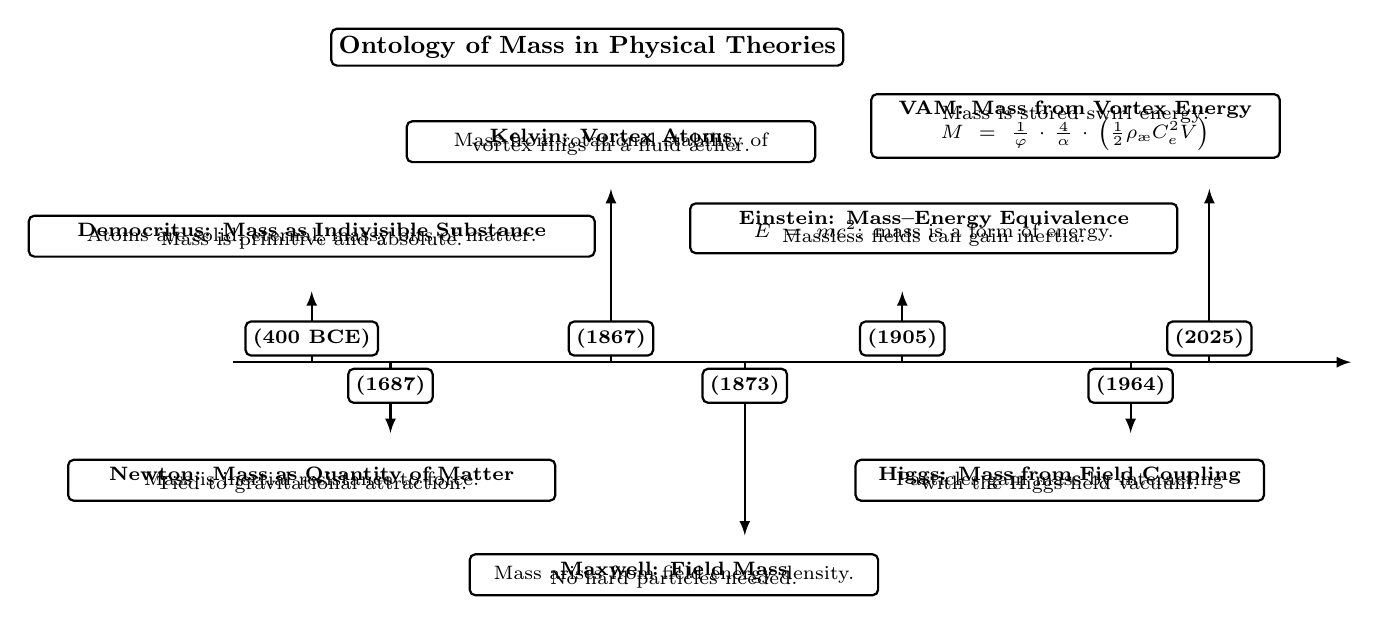
\begin{tikzpicture}[node distance=3.5cm, every node/.style={font=\scriptsize}, >=latex]
    \scriptsize

    % Timeline base
    \draw[->, thick] (-1,0) -- (13.2,0);

    % Arrows above timeline (short, as requested)
    \draw[->, thick] (0,0) -- (0,0.9);       % Pre-Socratics
    \draw[->, thick] (3.8,0) -- (3.8,2.2);   % Augustine
    \draw[->, thick] (7.5,0) -- (7.5,0.9);   % Einstein
    \draw[->, thick] (11.4,0) -- (11.4,2.2); % VAM

    % Arrows below timeline (short, as requested)
    \draw[->, thick] (1.0,0) -- (1.0,-0.9);     % Plato/Aristotle
    \draw[->, thick] (5.5,0) -- (5.5,-2.2);     % Newton
    \draw[->, thick] (10.4,0) -- (10.4,-0.9);     % Leibniz/Mach

        %--- Root title cards (above timeline) ---
    \node[draw, thick, rounded corners=2pt, fill=white, align=center, font=\bfseries ] at (0, .3)   {(400 BCE)};
    \node[draw, thick, rounded corners=2pt, fill=white, align=center, font=\bfseries ] at (3.8, .3) {(1867)};
    \node[draw, thick, rounded corners=2pt, fill=white, align=center, font=\bfseries ] at (7.5, .3) {(1905)};
    \node[draw, thick, rounded corners=2pt, fill=white, align=center, font=\bfseries ] at (11.4, .3){(2025)};

    %--- Root title cards (below timeline) ---
    \node[draw, thick, rounded corners=2pt, fill=white, align=center, font=\bfseries ] at (1.0,- .3) {(1687)};
    \node[draw, thick, rounded corners=2pt, fill=white, align=center, font=\bfseries ] at (5.5,- .3) {(1873)};
    \node[draw, thick, rounded corners=2pt, fill=white, align=center, font=\bfseries ] at (10.4,- .3) {(1964)};

    % Label
    \node[draw, thick, fill=white, rounded corners=2pt, font=\small] at (3.5,4.0) {\textbf{Ontology of Mass in Physical Theories}};

    % Democritus (left)
    \node[draw, rounded corners=2pt, thick, align=center, fill=white, text width=7cm] at (0,1.6) {
    \textbf{Democritus: Mass as Indivisible Substance}  \\[-0.8em]
    Atoms are solid, eternal, massy bits of matter.  \\[-0.8em]
    Mass is primitive and absolute.
    };

    % Newton (below)
    \node[draw, rounded corners=2pt, thick, align=center, fill=white, text width=6cm] at (0,-1.5) {
    \textbf{Newton: Mass as Quantity of Matter}  \\[-0.8em]
    Mass is inertial resistance to force.  \\[-0.8em]
    Tied to gravitational attraction.
    };


    % Kelvin (top)
    \node[draw, rounded corners=2pt, thick, align=center, fill=white, text width=5cm] at (3.8,2.8) {
    \textbf{Kelvin: Vortex Atoms}  \\[-0.8em]
    Mass from rotational stability of  \\[-0.8em]
    vortex rings in a fluid æther.
    };


    % Maxwell (bottom)
    \node[draw, rounded corners=2pt, thick, align=center, fill=white, text width=5cm] at (4.6,-2.7) {
    \textbf{Maxwell: Field Mass}  \\[-0.8em]
    Mass arises from field energy density.  \\[-0.8em]
    No hard particles needed.
    };

    % Einstein (top)
    \node[draw, rounded corners=2pt, thick, align=center, fill=white, text width=6cm] at (7.9,1.7) {
    \textbf{Einstein: Mass–Energy Equivalence}  \\[-0.4em]
    \( E = mc^2 \): mass is a form of energy.  \\[-0.8em]
    Massless fields can gain inertia.
    };


    % Higgs (bottom)
    \node[draw, rounded corners=2pt, thick, align=center, fill=white, text width=5cm] at (9.5,-1.5) {
    \textbf{Higgs: Mass from Field Coupling}  \\[-0.8em]
    Particles gain mass by interacting  \\[-0.8em]
    with the Higgs field vacuum.
    };


    % VAM (top right)
    \node[draw, rounded corners=2pt, thick, align=center, fill=white, text width=5cm] at (9.7,3.0) {
    \textbf{VAM: Mass from Vortex Energy}  \\[-0.8em]
    Mass is stored swirl energy:  \\[-0.4em]
    \( M = \frac{1}{\varphi} \cdot \frac{4}{\alpha} \cdot \left( \frac{1}{2} \rho_\text{\ae} C_e^2 V \right) \)
    };

    \end{tikzpicture}
    \caption{\textbf{Evolution of the concept of mass across physics:} from atomistic substance (Democritus), through Newtonian inertia and field-theoretic mass (Maxwell, Higgs), to VAM’s fluid-topological model. In VAM, mass is emergent swirl energy stored in knotted vortex configurations within a quantized æther. Each stage reflects deeper abstraction—from particles to energy to geometry to topology.}\label{fig:OntologyOfMass}
\end{figure}